\documentclass{beamer}

% Setup appearance:

%\usetheme{Darmstadt}
%\usetheme{Warsaw}
%\usetheme{Boadilla}
%\usetheme{Hannover}   %jó
%\usetheme{Marburg}      %jó
%\usetheme{Singapore}  %jó
%\usetheme{Szeged}
\usetheme{CambridgeUS}

%color theme
\usecolortheme{beaver}
%\usecolortheme{reen}


\usepackage[magyar]{babel}
%\usepackage[english]{babel}

\usepackage[utf8]{inputenc}
\usepackage{times}
\usepackage[T1]{fontenc}

\usepackage{amsmath}
\usepackage{graphicx}
\usepackage{enumerate}

\usepackage{caption}
%\usepackage{subcaption}

\usepackage{epstopdf}

\usepackage{color}
\usepackage{listings}
\definecolor{javared}{rgb}{0.6,0,0} % for strings
\definecolor{javagreen}{rgb}{0.25,0.5,0.35} % comments
\definecolor{javapurple}{rgb}{0.5,0,0.35} % keywords
\definecolor{javadocblue}{rgb}{0.25,0.35,0.75} % javadoc
 
\definecolor{dkgreen}{rgb}{0,.6,0}
\definecolor{dkblue}{rgb}{0,0,.6}
\definecolor{dkyellow}{cmyk}{0,0,.8,.3}

\lstset{
  language        = php,
  basicstyle      = \small\ttfamily,
  keywordstyle    = \color{dkblue},
  stringstyle     = \color{red},
  identifierstyle = \color{dkgreen},
  commentstyle    = \color{gray},
  emph            =[1]{php},
  emphstyle       =[1]\color{black},
  emph            =[2]{if,and,or,else},
  emphstyle       =[2]\color{dkyellow}}
 
%\lstset{language=Java,
%basicstyle=\ttfamily,
%keywordstyle=\color{javapurple}\bfseries,
%stringstyle=\color{javared},
%commentstyle=\color{javagreen},
%morecomment=[s][\color{javadocblue}]{/**}{*/},
%numbers=left,
%numberstyle=\tiny\color{black},
%stepnumber=2,
%numbersep=10pt,
%tabsize=4,
%showspaces=false,
%showstringspaces=false}
%\lstset{
%language=HTML,
%basicstyle=\ttfamily,
%keywordstyle=\color{blue},
%breaklines=true, 
%commentstyle=\color{javagreen},
%numbers=left,
%numberstyle=\tiny\color{gray},
%stepnumber=2,
%numbersep=5pt,
%}


\definecolor{okgreen}{rgb}{0,1,0}
\definecolor{wrongred}{rgb}{1,0,0}

\newcommand{\OK}{{\color{okgreen}\checkmark}}
\newcommand{\WRONG}{{\color{wrongred}X}}
\newcommand{\QUESTION}[1]{{\color{wrongred}¿} #1 {\color{wrongred}?}}
\newcommand{\QUESTIONMARK}{{\color{wrongred}?}}
\newcommand*{\supervisor}[1]{\def\supname{#1}}

% Author, Title, etc.

\title[Android Fejlesztés]{Szoftverfejlesztés Android platformra}

\author{Adam Satan}

\institute{Minőségbiztosítás informatikája}

\date{\the\year}

\begin{document}

\maketitle
%\begin{frame}
%  \titlepage
%\end{frame}

\section{Bevezető}

\begin{frame}[fragile]{Android}
	\begin{minipage}{0.49\textwidth}		
		\begin{itemize}
			\item Google - Android
			\item Android Studio
			\item Fejleszési nyelvek
			\item Szoftver fejlesztés
			\item Szoftver tesztelés	
		\end{itemize}
	\end{minipage}
\begin{minipage}{0.49\textwidth}

\includegraphics[width=1 \linewidth]{figures/android.png}
\end{minipage}
\end{frame}
\begin{frame}[fragile]{Google - Android}
	\begin{minipage}{0.49\textwidth}
		\begin{itemize}
			\item
		\end{itemize}
	\end{minipage}
	\begin{minipage}{0.49\textwidth}
		\begin{figure}
			\includegraphics[width=1\linewidth]{figures/beacon.png}
		\end{figure}
	\end{minipage}
\end{frame}
\begin{frame}[fragile]{Test Environment}
	\begin{minipage}{0.49\textwidth}
		\begin{itemize}
			\item Beacons
			\begin{itemize}
				\item Placed 12m apart
				\item In the ceiling for best coverage
			\end{itemize}
			\item Rooms
			\begin{itemize}
				\item Position
				\item Residents
			\end{itemize}
		\end{itemize}
	\end{minipage}
	\begin{minipage}{0.49\textwidth}
		\begin{figure}
			\includegraphics[width=0.7\linewidth]{figures/envir.png}
		\end{figure}
	\end{minipage}
\end{frame}
\section{Implementation}

\begin{frame}[fragile]{Application}
	\begin{minipage}{0.49\textwidth}
		\begin{itemize}
			\item Developed for Android
			\item Implemented in Java
			\item Utilizes Bluetooth Low Energy technology
		\end{itemize}
	\end{minipage}
	\begin{minipage}{0.49\textwidth}
		\begin{figure}
			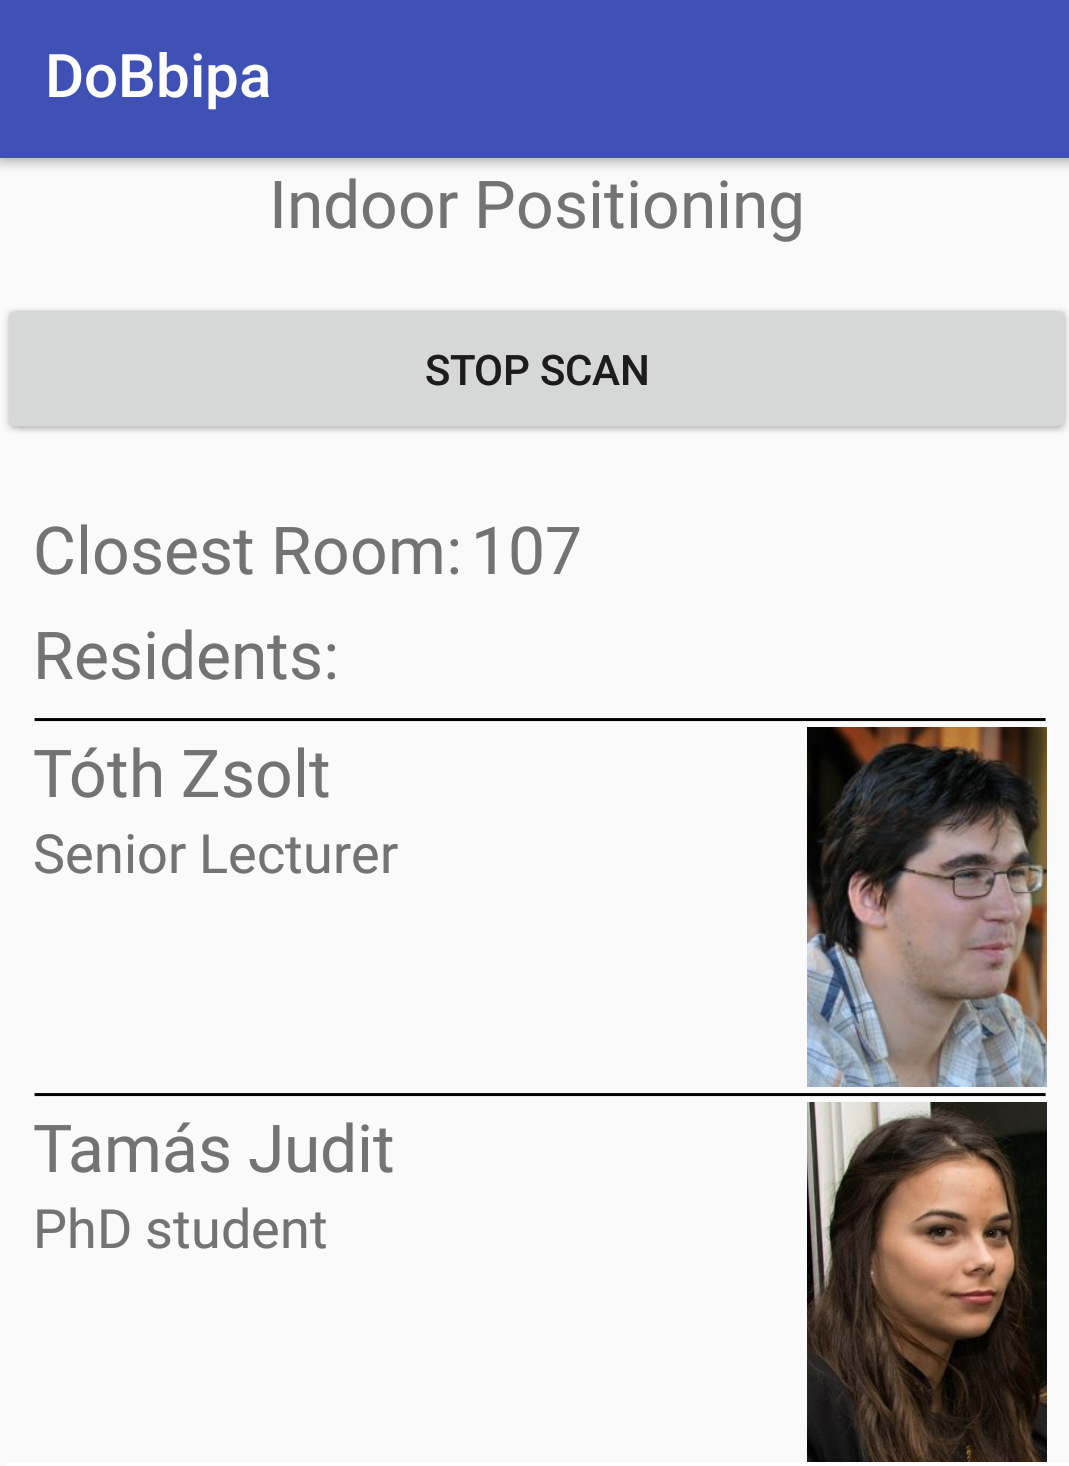
\includegraphics[width=1\linewidth]{figures/app2.png}
		\end{figure}
	\end{minipage}
\end{frame}
\section{Method}
\begin{frame}[fragile]{Algorithm}
\begin{minipage}{0.49\textwidth}
\begin{itemize}
	\item Get RSSI
	\item Filter RSSI
	\item Calculate distance 
	 $d=exp(\dfrac{RSSI - A_{0}}{-10n})$
	\item Calculate distance between positions
	\item Determine User Position
	\item Find Closest room
\end{itemize}
\end{minipage}
\begin{minipage}{0.49\textwidth}
\begin{figure}
	\includegraphics[width=1\linewidth]{figures/pitagorasz.png}
\end{figure}
\end{minipage}
\end{frame}

\section{Cases}
\begin{frame}[fragile]{Case 1}
	\begin{minipage}{0.49\textwidth}
		\begin{itemize}
			\item User Between Beacons
			\item Relies on both
			\item Proportional Division
			\item Device independent solution
		\end{itemize}
	\end{minipage}
	\begin{minipage}{0.49\textwidth}
		\begin{figure}
			\includegraphics[width=1\linewidth]{figures/test222.png}
		\end{figure}
	\end{minipage}
\end{frame}
\begin{frame}[fragile]{Case 2}
\begin{minipage}{0.49\textwidth}
\begin{itemize}
	\item User isn't between beacons
	\item Relies on the closest Beacon
	\item Places the user on the beaconless side
	\item Different results in different devices
\end{itemize}
\end{minipage}
\begin{minipage}{0.49\textwidth}
\begin{figure}
	\includegraphics[width=1\linewidth]{figures/test111.png}
\end{figure}
\end{minipage}
\end{frame}



\section{Result}



\begin{frame}[fragile]{Test Results}

	\begin{minipage}{1\textwidth}
		\begin{table}[h]
			\centering
%			\caption{Test Results}\label{tab:testResutls}
			\begin{tabular}{|c|c|c|c|}
				\hline
				Reference point & Position & Correct & Not correct\\ 
				\hline 
				(4,7) outside beacons & 107 & 7 & 0 \\ \hline
				(6,7) under beacon 1 & 107 & 7 & 0 \\ \hline
				(10,7) front of fire hose & 108 & 6 & 1 \\ \hline
				(14,7) front of room 108 & 108 & 7 & 0 \\ \hline
				(16,7) between room 108 and 123 & 108 & 3 & 4 \\ \hline
				(18,7) under beacon 2 & 123 & 7 & 0\\ \hline
				
			\end{tabular}
		\end{table}
	\end{minipage}
%	\begin{minipage}{0.42\textheight}
%		\includegraphics[width=1\linewidth]{figures/measuresss.png}
%	\end{minipage}
\end{frame}

\begin{frame}[fragile]{Discussion}
	\begin{minipage}{0.39\textwidth}
		\begin{itemize}
			\item Overall 88\% accuracy
			\item Human body
			\item WiFi interference
			\item Increased Beacon density
		\end{itemize}
	\end{minipage}
	\begin{minipage}{0.59\textwidth}
		\begin{itemize}
			\item Future plans
			\begin{itemize}
				\item Navigation
				\item Orientation consideration
				\item Dead Reckoning technique 
				\item ILONA integration
			\end{itemize}
		\end{itemize}
	\end{minipage}
\end{frame}




\section{}
\begin{frame}
\centering
\LARGE Thank you for your attention!
\end{frame}

\end{document} 